%
% 6.006 problem set 5 solutions template
%
\documentclass[12pt,twoside]{article}

\newcommand{\name}{}

\usepackage{amssymb}
\usepackage{amsmath}
\usepackage{graphicx}
\usepackage{latexsym}
\usepackage{times,url}
\usepackage{cprotect}
\usepackage{listings}
\usepackage{graphicx}
\usepackage[table]{xcolor}
\usepackage[letterpaper]{geometry}
\usepackage{tikz-qtree}
\usepackage{enumerate}

\newcommand{\profs}{Instructors: Erik Demaine, Jason Ku, and Justin Solomon}
\newcommand{\subj}{6.006}
\newcommand{\ttt}[1]{{\tt\small #1}}

\definecolor{dkgreen}{rgb}{0,0.6,0}
\definecolor{dkblue}{rgb}{.2,.2,1}
\definecolor{gray}{rgb}{0.5,0.5,0.5}
\definecolor{mauve}{rgb}{0.58,0,0.82}

\lstset{
  language=Python,
  aboveskip=1pc,
  belowskip=1pc,
  basicstyle={\footnotesize\ttfamily},
  numbers=left,
  showstringspaces=false,
  numberstyle={\tiny\color{gray}\ttfamily},
  keywordstyle={\color{dkblue}\ttfamily},
  commentstyle={\color{dkgreen}\ttfamily},
  stringstyle={\color{mauve}\ttfamily},
}

% \lstset{
%   language=Python,
%   aboveskip=1pc,
%   belowskip=1pc,
%   basicstyle={\bf\color{white}\ttfamily},
%   numbers=left,
%   showstringspaces=false,
%   numberstyle={\bf\small\color{lightgray}\ttfamily},
%   keywordstyle={\bf\color{cyan}\ttfamily},
%   commentstyle={\bf\color{green}\ttfamily},
%   stringstyle={\bf\color{mauve}\ttfamily},
% }

\tikzset{
  % every node/.style={minimum width=2em,draw,circle},
  % level 1/.style={sibling distance=2cm},
  level distance=1cm,
  edge from parent/.style=
  {draw,edge from parent path={(\tikzparentnode) -- (\tikzchildnode)}},
}
\usetikzlibrary{shapes}

\newif\ifHideSolutions
\newcommand{\solution}[1]{\color{dkgreen}\textbf{Solution: }#1\color{black}}
\newcommand{\commonmistakes}[1]{{\color{dkblue}\textbf{Common Mistakes: }#1}}
\newcommand{\rubric}[1]{\color{dkgreen}{\bf Rubric:} #1\color{black}}

% \HideSolutionsfalse
% \ifHideSolutions
%   \renewcommand{\solution}[1]{}
%   \renewcommand{\rubric}[1]{}
% \fi

\newlength{\toppush}
\setlength{\toppush}{2\headheight}
\addtolength{\toppush}{\headsep}

\newcommand{\htitle}[2]{\noindent\vspace*{-\toppush}\newline\parbox{\textwidth}
{\textit{Introduction to Algorithms: 6.006}\hfill\name\newline
Massachusetts Institute of Technology \hfill #2\newline
\profs\hfill #1 \\[-3.5ex]\newline
\mbox{}\hrulefill\mbox{}}\vspace*{1ex}\mbox{}\newline
\begin{center}{\Large\bf #1}\end{center}}

\newcommand{\handout}[2]{\thispagestyle{empty}
 \markboth{#1}{#1}
 \pagestyle{myheadings}\htitle{#1}{#2}}

\newcommand{\lecture}[3]{\thispagestyle{empty}
 \markboth{Lecture #1: #2}{Lecture #1: #2}
 \pagestyle{myheadings}\htitle{Lecture #1: #2}{#3}}

\newcommand{\htitlewithouttitle}[2]{\noindent\vspace*{-\toppush}\newline\parbox{6.5in}
{\textit{Introduction to Algorithms}\hfill#2\newline
Massachusetts Institute of Technology \hfill 6.006\newline
\profs\hfill Handout #1\vspace*{-.5ex}\newline
\mbox{}\hrulefill\mbox{}}\vspace*{1ex}\mbox{}\newline}

\newcommand{\handoutwithouttitle}[2]{\thispagestyle{empty}
 \markboth{Handout \protect\ref{#1}}{Handout \protect\ref{#1}}
 \pagestyle{myheadings}\htitlewithouttitle{\protect\ref{#1}}{#2}}

\newcommand{\exam}[2]{% parameters: exam name, date
 \thispagestyle{empty}
 \markboth{\hspace{1cm}\subj\ #1\hspace{1in}Name\hrulefill\ \ }%
          {\subj\ #1\hspace{1in}Name\hrulefill\ \ }
 \pagestyle{myheadings}\examtitle{#1}{#2}
 \renewcommand{\theproblem}{Problem \arabic{problemnum}}
}
\newcommand{\examsolutions}[3]{% parameters: handout, exam name, date
 \thispagestyle{empty}
 \markboth{Handout \protect\ref{#1}: #2}{Handout \protect\ref{#1}: #2}
% \pagestyle{myheadings}\htitle{\protect\ref{#1}}{#2}{#3}
 \pagestyle{myheadings}\examsolutionstitle{\protect\ref{#1}} {#2}{#3}
 \renewcommand{\theproblem}{Problem \arabic{problemnum}}
}
\newcommand{\examsolutionstitle}[3]{\noindent\vspace*{-\toppush}\newline\parbox{6.5in}
{\textit{Introduction to Algorithms}\hfill#3\newline
Massachusetts Institute of Technology \hfill 6.006\newline
%Singapore-MIT Alliance \hfill SMA5503\newline
\profs\hfill Handout #1\vspace*{-.5ex}\newline
\mbox{}\hrulefill\mbox{}}\vspace*{1ex}\mbox{}\newline
\begin{center}{\Large\bf #2}\end{center}}

\newcommand{\takehomeexam}[2]{% parameters: exam name, date
 \thispagestyle{empty}
 \markboth{\subj\ #1\hfill}{\subj\ #1\hfill}
 \pagestyle{myheadings}\examtitle{#1}{#2}
 \renewcommand{\theproblem}{Problem \arabic{problemnum}}
}

\makeatletter
\newcommand{\exambooklet}[2]{% parameters: exam name, date
 \thispagestyle{empty}
 \markboth{\subj\ #1}{\subj\ #1}
 \pagestyle{myheadings}\examtitle{#1}{#2}
 \renewcommand{\theproblem}{Problem \arabic{problemnum}}
 \renewcommand{\problem}{\newpage
 \item \let\@currentlabel=\theproblem
 \markboth{\subj\ #1, \theproblem}{\subj\ #1, \theproblem}}
}
\makeatother


\newcommand{\examtitle}[2]{\noindent\vspace*{-\toppush}\newline\parbox{6.5in}
{\textit{Introduction to Algorithms}\hfill#2\newline
Massachusetts Institute of Technology \hfill 6.006 Spring 2020\newline
%Singapore-MIT Alliance \hfill SMA5503\newline
\profs\hfill #1\vspace*{-.5ex}\newline
\mbox{}\hrulefill\mbox{}}\vspace*{1ex}\mbox{}\newline
\begin{center}{\Large\bf #1}\end{center}}

\newcommand{\grader}[1]{\hspace{1cm}\textsf{\textbf{#1}}\hspace{1cm}}

\newcommand{\points}[1]{[#1 points]\ }
\newcommand{\parts}[1]
{
  \ifnum#1=1
  (1 part)
  \else
  (#1 parts)
  \fi
  \ 
}

\newcommand{\bparts}{\begin{problemparts}}
\newcommand{\eparts}{\end{problemparts}}
\newcommand{\ppart}{\problempart}

%\newcommand{\lg} {lg\ }

\setlength{\oddsidemargin}{0pt}
\setlength{\evensidemargin}{0pt}
\setlength{\textwidth}{6.5in}
\setlength{\topmargin}{0in}
\setlength{\textheight}{8.5in}


\newcommand{\Spawn}{{\bf spawn} }
\newcommand{\Sync}{{\bf sync}}

\renewcommand{\cases}[1]{\left\{ \begin{array}{ll}#1\end{array}\right.}
\newcommand{\cif}[1]{\mbox{if $#1$}}
\newcommand{\cwhen}[1]{\mbox{when $#1$}}

\newcounter{problemnum}
\newcommand{\theproblem}{Problem \theproblemsetnum-\arabic{problemnum}}
\newenvironment{problems}{
        \begin{list}{{\bf \theproblem. \hspace*{0.5em}}}
        {\setlength{\leftmargin}{0em}
         \setlength{\rightmargin}{0em}
         \setlength{\labelwidth}{0em}
         \setlength{\labelsep}{0em}
         \usecounter{problemnum}}}{\end{list}}
\makeatletter
\newcommand{\problem}[1][{}]{\item \let\@currentlabel=\theproblem \textbf{#1}}
\makeatother

\newcounter{problempartnum}[problemnum]
\newenvironment{problemparts}{
        \begin{list}{{\bf (\alph{problempartnum})}}
        {\setlength{\leftmargin}{2.5em}
         \setlength{\rightmargin}{2.5em}
         \setlength{\labelsep}{0.5em}}}{\end{list}}
\newcommand{\problempart}{\addtocounter{problempartnum}{1}\item}

\newenvironment{truefalseproblemparts}{
        \begin{list}{{\bf (\alph{problempartnum})\ \ \ T\ \ F\hfil}}
        {\setlength{\leftmargin}{4.5em}
         \setlength{\rightmargin}{2.5em}
         \setlength{\labelsep}{0.5em}
         \setlength{\labelwidth}{4.5em}}}{\end{list}}

\newcounter{exercisenum}
\newcommand{\theexercise}{Exercise \theproblemsetnum-\arabic{exercisenum}}
\newenvironment{exercises}{
        \begin{list}{{\bf \theexercise. \hspace*{0.5em}}}
        {\setlength{\leftmargin}{0em}
         \setlength{\rightmargin}{0em}
         \setlength{\labelwidth}{0em}
         \setlength{\labelsep}{0em}
        \usecounter{exercisenum}}}{\end{list}}
\makeatletter
\newcommand{\exercise}{\item \let\@currentlabel=\theexercise}
\makeatother

\newcounter{exercisepartnum}[exercisenum]
%\newcommand{\problem}[1]{\medskip\mbox{}\newline\noindent{\bf Problem #1.}\hspace*{1em}}
%\newcommand{\exercise}[1]{\medskip\mbox{}\newline\noindent{\bf Exercise #1.}\hspace*{1em}}

\newenvironment{exerciseparts}{
        \begin{list}{{\bf (\alph{exercisepartnum})}}
        {\setlength{\leftmargin}{2.5em}
         \setlength{\rightmargin}{2.5em}
         \setlength{\labelsep}{0.5em}}}{\end{list}}
\newcommand{\exercisepart}{\addtocounter{exercisepartnum}{1}\item}


% Macros to make captions print with small type and 'Figure xx' in bold.
\makeatletter
\def\fnum@figure{{\bf Figure \thefigure}}
\def\fnum@table{{\bf Table \thetable}}
\let\@mycaption\caption
%\long\def\@mycaption#1[#2]#3{\addcontentsline{\csname
%  ext@#1\endcsname}{#1}{\protect\numberline{\csname 
%  the#1\endcsname}{\ignorespaces #2}}\par
%  \begingroup
%    \@parboxrestore
%    \small
%    \@makecaption{\csname fnum@#1\endcsname}{\ignorespaces #3}\par
%  \endgroup}
%\def\mycaption{\refstepcounter\@captype \@dblarg{\@mycaption\@captype}}
%\makeatother
\let\mycaption\caption
%\newcommand{\figcaption}[1]{\mycaption[]{#1}}

\newcounter{totalcaptions}
\newcounter{totalart}

\newcommand{\figcaption}[1]{\addtocounter{totalcaptions}{1}\caption[]{#1}}

% \psfigures determines what to do for figures:
%       0 means just leave vertical space
%       1 means put a vertical rule and the figure name
%       2 means insert the PostScript version of the figure
%       3 means put the figure name flush left or right
\newcommand{\psfigures}{0}
\newcommand{\spacefigures}{\renewcommand{\psfigures}{0}}
\newcommand{\rulefigures}{\renewcommand{\psfigures}{1}}
\newcommand{\macfigures}{\renewcommand{\psfigures}{2}}
\newcommand{\namefigures}{\renewcommand{\psfigures}{3}}

\newcommand{\figpart}[1]{{\bf (#1)}\nolinebreak[2]\relax}
\newcommand{\figparts}[2]{{\bf (#1)--(#2)}\nolinebreak[2]\relax}


\macfigures     % STATE

% When calling \figspace, make sure to leave a blank line afterward!!
% \widefigspace is for figures that are more than 28pc wide.
\newlength{\halffigspace} \newlength{\wholefigspace}
\newlength{\figruleheight} \newlength{\figgap}
\newcommand{\setfiglengths}{\ifnum\psfigures=1\setlength{\figruleheight}{\hruleheight}\setlength{\figgap}{1em}\else\setlength{\figruleheight}{0pt}\setlength{\figgap}{0em}\fi}
\newcommand{\figspace}[2]{\ifnum\psfigures=0\leavefigspace{#1}\else%
\setfiglengths%
\setlength{\wholefigspace}{#1}\setlength{\halffigspace}{.5\wholefigspace}%
\rule[-\halffigspace]{\figruleheight}{\wholefigspace}\hspace{\figgap}#2\fi}
\newlength{\widefigspacewidth}
% Make \widefigspace put the figure flush right on the text page.
\newcommand{\widefigspace}[2]{
\ifnum\psfigures=0\leavefigspace{#1}\else%
\setfiglengths%
\setlength{\widefigspacewidth}{28pc}%
\addtolength{\widefigspacewidth}{-\figruleheight}%
\setlength{\wholefigspace}{#1}\setlength{\halffigspace}{.5\wholefigspace}%
\makebox[\widefigspacewidth][r]{#2\hspace{\figgap}}\rule[-\halffigspace]{\figruleheight}{\wholefigspace}\fi}
\newcommand{\leavefigspace}[1]{\setlength{\wholefigspace}{#1}\setlength{\halffigspace}{.5\wholefigspace}\rule[-\halffigspace]{0em}{\wholefigspace}}

% Commands for including figures with macpsfig.
% To use these commands, documentstyle ``macpsfig'' must be specified.
\newlength{\macfigfill}
\makeatother
\newlength{\bbx}
\newlength{\bby}
\newcommand{\macfigure}[5]{\addtocounter{totalart}{1}
\ifnum\psfigures=2%
\setlength{\bbx}{#2}\addtolength{\bbx}{#4}%
\setlength{\bby}{#3}\addtolength{\bby}{#5}%
\begin{flushleft}
\ifdim#4>28pc\setlength{\macfigfill}{#4}\addtolength{\macfigfill}{-28pc}\hspace*{-\macfigfill}\fi%
\mbox{\psfig{figure=./#1.ps,%
bbllx=#2,bblly=#3,bburx=\bbx,bbury=\bby}}
\end{flushleft}%
\else\ifdim#4>28pc\widefigspace{#5}{#1}\else\figspace{#5}{#1}\fi\fi}
\makeatletter

\newlength{\savearraycolsep}
\newcommand{\narrowarray}[1]{\setlength{\savearraycolsep}{\arraycolsep}\setlength{\arraycolsep}{#1\arraycolsep}}
\newcommand{\normalarray}{\setlength{\arraycolsep}{\savearraycolsep}}

\newcommand{\hint}{{\bf Hint:\ }}

% Macros from /th/u/clr/mac.tex

\newcommand{\set}[1]{\left\{ #1 \right\}}
\newcommand{\abs}[1]{\left| #1\right|}
\newcommand{\card}[1]{\left| #1\right|}
\newcommand{\floor}[1]{\left\lfloor #1 \right\rfloor}
\newcommand{\ceil}[1]{\left\lceil #1 \right\rceil}
\newcommand{\ang}[1]{\ifmmode{\left\langle #1 \right\rangle}
   \else{$\left\langle${#1}$\right\rangle$}\fi}
        % the \if allows use outside mathmode,
        % but will swallow following space there!
\newcommand{\paren}[1]{\left( #1 \right)}
\newcommand{\bracket}[1]{\left[ #1 \right]}
\newcommand{\prob}[1]{\Pr\left\{ #1 \right\}}
\newcommand{\Var}{\mathop{\rm Var}\nolimits}
\newcommand{\expect}[1]{{\rm E}\left[ #1 \right]}
\newcommand{\expectsq}[1]{{\rm E}^2\left[ #1 \right]}
\newcommand{\variance}[1]{{\rm Var}\left[ #1 \right]}
\renewcommand{\choose}[2]{{{#1}\atopwithdelims(){#2}}}
\def\pmod#1{\allowbreak\mkern12mu({\rm mod}\,\,#1)}
\newcommand{\matx}[2]{\left(\begin{array}{*{#1}{c}}#2\end{array}\right)}
\newcommand{\Adj}{\mathop{\rm Adj}\nolimits}

\newtheorem{theorem}{Theorem}
\newtheorem{lemma}[theorem]{Lemma}
\newtheorem{corollary}[theorem]{Corollary}
\newtheorem{xample}{Example}
\newtheorem{definition}{Definition}
\newenvironment{example}{\begin{xample}\rm}{\end{xample}}
\newcommand{\proof}{\noindent{\em Proof.}\hspace{1em}}
\def\squarebox#1{\hbox to #1{\hfill\vbox to #1{\vfill}}}
\newcommand{\qedbox}{\vbox{\hrule\hbox{\vrule\squarebox{.667em}\vrule}\hrule}}
\newcommand{\qed}{\nopagebreak\mbox{}\hfill\qedbox\smallskip}
\newcommand{\eqnref}[1]{(\protect\ref{#1})}

%%\newcommand{\twodots}{\mathinner{\ldotp\ldotp}}
\newcommand{\transpose}{^{\mbox{\scriptsize \sf T}}}
\newcommand{\amortized}[1]{\widehat{#1}}

\newcommand{\punt}[1]{}

%%% command for putting definitions into boldface
% New style for defined terms, as of 2/23/88, redefined by THC.
\newcommand{\defn}[1]{{\boldmath\textit{\textbf{#1}}}}
\newcommand{\defi}[1]{{\textit{\textbf{#1\/}}}}

\newcommand{\red}{\leq_{\rm P}}
\newcommand{\lang}[1]{%
\ifmmode\mathord{\mathcode`-="702D\rm#1\mathcode`\-="2200}\else{\rm#1}\fi}

%\newcommand{\ckt}[1]{\ifmmode\mathord{\mathcode`-="702D\sc #1\mathcode`\-="2200}\else$\mathord{\mathcode`-="702D\sc #1\mathcode`\-="2200}$\fi}
\newcommand{\ckt}[1]{\ifmmode \sc #1\else$\sc #1$\fi}

%% Margin notes - use \notesfalse to turn off notes.
\setlength{\marginparwidth}{0.6in}
\reversemarginpar
\newif\ifnotes
\notestrue
\newcommand{\longnote}[1]{
  \ifnotes
    {\medskip\noindent Note: \marginpar[\hfill$\Longrightarrow$]
      {$\Longleftarrow$}{#1}\medskip}
  \fi}
\newcommand{\note}[1]{
  \ifnotes
    {\marginpar{\tiny \raggedright{#1}}}
  \fi}


\newcommand{\reals}{\mathbbm{R}}
\newcommand{\integers}{\mathbbm{Z}}
\newcommand{\naturals}{\mathbbm{N}}
\newcommand{\rationals}{\mathbbm{Q}}
\newcommand{\complex}{\mathbbm{C}}

\newcommand{\oldreals}{{\bf R}}
\newcommand{\oldintegers}{{\bf Z}}
\newcommand{\oldnaturals}{{\bf N}}
\newcommand{\oldrationals}{{\bf Q}}
\newcommand{\oldcomplex}{{\bf C}}

\newcommand{\w}{\omega}                 %% for fft chapter

\newenvironment{closeitemize}{\begin{list}
{$\bullet$}
{\setlength{\itemsep}{-0.2\baselineskip}
\setlength{\topsep}{0.2\baselineskip}
\setlength{\parskip}{0pt}}}
{\end{list}}

% These are necessary within a {problems} environment in order to restore
% the default separation between bullets and items.
\newenvironment{normalitemize}{\setlength{\labelsep}{0.5em}\begin{itemize}}
                              {\end{itemize}}
\newenvironment{normalenumerate}{\setlength{\labelsep}{0.5em}\begin{enumerate}}
                                {\end{enumerate}}

%\def\eqref#1{Equation~(\ref{eq:#1})}
%\newcommand{\eqref}[1]{Equation (\ref{eq:#1})}
\newcommand{\eqreftwo}[2]{Equations (\ref{eq:#1}) and~(\ref{eq:#2})}
\newcommand{\ineqref}[1]{Inequality~(\ref{ineq:#1})}
\newcommand{\ineqreftwo}[2]{Inequalities (\ref{ineq:#1}) and~(\ref{ineq:#2})}

\newcommand{\figref}[1]{Figure~\ref{fig:#1}}
\newcommand{\figreftwo}[2]{Figures \ref{fig:#1} and~\ref{fig:#2}}

\newcommand{\liref}[1]{line~\ref{li:#1}}
\newcommand{\Liref}[1]{Line~\ref{li:#1}}
\newcommand{\lirefs}[2]{lines \ref{li:#1}--\ref{li:#2}}
\newcommand{\Lirefs}[2]{Lines \ref{li:#1}--\ref{li:#2}}
\newcommand{\lireftwo}[2]{lines \ref{li:#1} and~\ref{li:#2}}
\newcommand{\lirefthree}[3]{lines \ref{li:#1}, \ref{li:#2}, and~\ref{li:#3}}

\newcommand{\lemlabel}[1]{\label{lem:#1}}
\newcommand{\lemref}[1]{Lemma~\ref{lem:#1}} 

\newcommand{\exref}[1]{Exercise~\ref{ex:#1}}

\newcommand{\handref}[1]{Handout~\ref{#1}}

\newcommand{\defref}[1]{Definition~\ref{def:#1}}

% (1997.8.16: Victor Luchangco)
% Modified \hlabel to only get date and to use handouts counter for number.
%   New \handout and \handoutwithouttitle commands in newmac.tex use this.
%   The date is referenced by <label>-date.
%   (Retained old definition as \hlabelold.)
%   Defined \hforcelabel to use an argument instead of the handouts counter.

\newcounter{handouts}
\setcounter{handouts}{0}

\newcommand{\hlabel}[2]{%
\stepcounter{handouts}
{\edef\next{\write\@auxout{\string\newlabel{#1}{{\arabic{handouts}}{0}}}}\next}
\write\@auxout{\string\newlabel{#1-date}{{#2}{0}}}
}

\newcommand{\hforcelabel}[3]{%          Does not step handouts counter.
\write\@auxout{\string\newlabel{#1}{{#2}{0}}}
\write\@auxout{\string\newlabel{#1-date}{{#3}{0}}}}


% less ugly underscore
% --juang, 2008 oct 05
\renewcommand{\_}{\vrule height 0 pt depth 0.4 pt width 0.5 em \,}

% multiline framed box (will always extend to the far right edge; for a short single line, use \fbox directly)
% --zabel, fall 2018
\newcommand\framepar[1]{\fbox{\begin{minipage}{\linewidth}#1\end{minipage}}}


\newcommand{\theproblemsetnum}{5}

\title{6.006 Problem Set \theproblemsetnum}

\begin{document}

\handout{Problem Set \theproblemsetnum}

\setlength{\parindent}{0pt}
\medskip\hrulefill\medskip

{\bf Name:} Gabriel Chiong

\medskip

{\bf Collaborators:} None

\medskip\hrulefill

%%%%%%%%%%%%%%%%%%%%%%%%%%%%%%%%%%%%%%%%%%%%%%%%%%%%%
% See below for common and useful latex constructs. %
%%%%%%%%%%%%%%%%%%%%%%%%%%%%%%%%%%%%%%%%%%%%%%%%%%%%%

% Some useful commands:
%$f(x) = \Theta(x)$
%$T(x, y) \leq \log(x) + 2^y + \binom{2n}{n}$
% {\tt code\_function}


% You can create unnumbered lists as follows:
%\begin{itemize}
%    \item First item in a list
%        \begin{itemize}
%            \item First item in a list
%                \begin{itemize}
%                    \item First item in a list
%                    \item Second item in a list
%                \end{itemize}
%            \item Second item in a list
%        \end{itemize}
%    \item Second item in a list
%\end{itemize}

% You can create numbered lists as follows:
%\begin{enumerate}
%    \item First item in a list
%    \item Second item in a list
%    \item Third item in a list
%\end{enumerate}

% You can write aligned equations as follows:
%\begin{align}
%    \begin{split}
%        (x+y)^3 &= (x+y)^2(x+y) \\
%                &= (x^2+2xy+y^2)(x+y) \\
%                &= (x^3+2x^2y+xy^2) + (x^2y+2xy^2+y^3) \\
%                &= x^3+3x^2y+3xy^2+y^3
%    \end{split}
%\end{align}

% You can create grids/matrices as follows:
%\begin{align}
%    A =
%    \begin{bmatrix}
%        A_{11} & A_{21} \\
%        A_{21} & A_{22}
%    \end{bmatrix}
%\end{align}

% You can include images and PDFs as follows:
% 
\includegraphics[width=0.5\textwidth]{img.jpg}

\begin{problems}

\problem  % Problem 1

\begin{problemparts}
\problempart % Problem 1a
Answer:

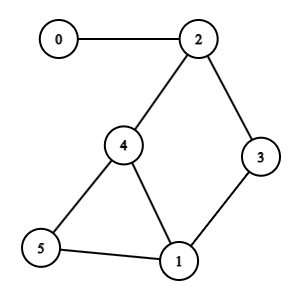
\includegraphics[width=0.3\textwidth]{tex/ps5/1a.png}

\problempart % Problem 1b
\begin{verbatim}
Adj = {
    'A': ['B'],
    'B': ['C', 'D'],
    'C': ['E', 'F'],
    'D': ['E', 'F'],
    'E': [],
    'F': ['D', 'E']
}
\end{verbatim}

\problempart % Problem 1c
BFS: A, B, C, D, E, F

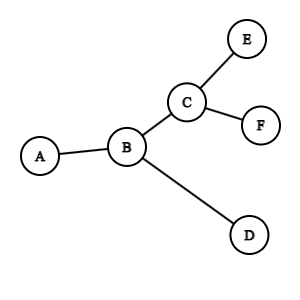
\includegraphics[width=0.3\textwidth]{tex/ps5/1c1.png}

DFS: A, B, C, E, F, D

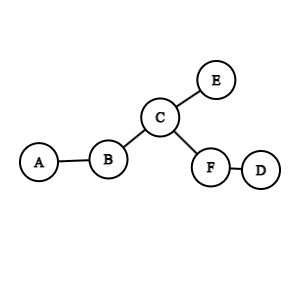
\includegraphics[width=0.3\textwidth]{tex/ps5/1c2.png}

\problempart % Problem 1d
There is only one cycle in the graph, therefore removing either $(D, F)$ or $(F, D)$ would result in a DAG.

If we remove edge $(F, D)$, there are two valid topological orderings, based on running DFS: \verb|[A, B, D, C, F, E]| and \verb|[A, B, C, D, F, E]|.

If we remove edge $(D, F)$, there is a unique topological ordering from running DFS: \verb|[A, B, C, F, D, E]|.

\end{problemparts}

\newpage
\problem  % Problem 2
If we construct a graph $G$ with plants and buildings as vertices and wires as edges, this problem is equivalent to finding the largest connected component (by vertex count). We know that each plant belongs to at most one connected component since each building is powered by no more than one plant. Therefore, the plant belonging to the largest connected component should receive the backup generator.

Graph $G$ has $n^2 + n$ vertices (number of buildings and number of plants). Therefore $|E|$ is upper-bounded by $O(n^2+n)=O(n^4)$ as required by the problem, since there is at most one wire connecting each pair of vertices.

The algorithm proceeds by running Full-BFS or Full-DFS to count the size of each connected component and return the largest connected component's plant. Constructing $G$ takes $O(n^4)$, running Full-BFS or Full-DFS takes $O(n^4)$, and iterating over the connected components to find the largest count takes $O(n)$ time. Therefore, the entire algorithm runs in $O(n^4)$ time as required.

\newpage
\problem  % Problem 3
Construct a (potentially disconnected) undirected graph $G$, with each vertex representing a friend in the $n$-length short-circuiting pairs list, and an edge between any pair of vertices of short-circuiting friend vertices.

The problem of determining whether two parties are sufficient for inviting all their friends is then equivalent to finding a 2-coloring of graph $G$. Each color represents a party, and if adjacent vertices can be divided into two sets, then two parties is possible. If there is an odd-cycle in the graph (two adjacent vertices have the same color; two short-circuiting friends attending the same party), then more than two parties will be needed.

The algorithm is to run Full-BFS on $G$ to obtain the shortest path distances from an arbitrary starting vertex from each connected component. Along the way, assign each vertex one of two colors, with all even-length shortest distances being of the same color, and all odd-length shortest distances being of another color. Next, iterate over all edges of the graph, and for each edge check if both adjacent vertices are of different color. If there is at least one pair of adjacent vertices with the same color, then return that two parties is not sufficient. Otherwise, at the end of iterating through all edges in $G$, return that two parties is possible.

$G$ has $n$ edges, and at most $2n$ vertices. Therefore it takes at most $O(n)$ time to construct. Using Full-BFS to color the vertices takes $O(|V|+|E|)=O(2n+n)=O(n)$ time, and iterating over edges takes $O(n)$ time (since there is only a constant amount of work to check each edge). Therefore, the algorithm runs in $O(n)$ time in the worst-case.

\newpage
\problem  % Problem 4
Let $M$ be the $n \times n$ labeled map, where $M[r][c]$ is the label of the grid square in row $r$ and column $c$. Construct a graph $G$ with $(n+1)^2$ vertices, where each vertex is labeled $(r,c)$ for all $r, c \in \{0, \ldots,n\}$. We place an undirected edge between two vertices under two scenarios.

Firstly, between vertices $(r, c-1)$ to $(r, c)$; left to right of the map, on the condition that $r$ is not a boundary edge (i.e. $r \in \{0,n\}$ is true) and $M[r][c-1]\neq M[r][c]$ (edge does not go between two squares owned by the same farmer).

Secondly, between vertices $(r-1,c)$ to $(r,c)$; top to bottom of the map, on the condition that $c$ is not a boundary edge (i.e. $c \in \{0,n\}$ is true) and $M[r-1][c] \neq M[r][c]$ (edge does not go between two squares owned by the same farmer).

This graph has the property that a path between two vertices corresponds to a route on the map that does not trample crops. For each square $M[r][c]$ that is part of the Euphris river, mark the vertices $(r,c),(r+1,c),(r,c+1),(r+1,c+1)$ as "Euphris squares". Do likewise with squares belonging to the Tigrates river.

Using BFS on each of the $\Omega(n^2)$ Euphris-labeled vertex would incur a time complexity of $\Omega(n^2)$ for each run of BFS. This exceeds the specified time complexity of the required algorithm. Therefore, add a supernode $s$ to $G$ with an undirected edge to each Euphris-labeled vertex to construct graph $G'$. Now any possible trade route will correspond to a path from $s$ to a Tigres-labeled vertex in $G'$ (discounting the supernode), and return the shortest path to any Tigres-labeled vertex by traversing parent pointers back to the source.

Graph $G'$ has $(n+1)^2+1$ vertices (including the supernode), and $O(n^2)+O(n^2)$ edges, so can be constructed in $O(n^2)$ time. Running BFS once from $s$ also takes $O(n^2)$ time, so this algorithm runs in $O(n^2)$ time overall.

\newpage
\problem  % Problem 5
Since the doors that Liza can enter depends on which key cards she currently has, we use graph duplication to enumerate the different scenarios along her journey. Since there are four types of key cards, there are at most $2^4=O(1)$ different possible states from key cards. At any location, there is also either a pizza or not, which gives $2^2=O(1)$ different possibilities. We therefore construct a graph $G$ with $2^5$ vertices, representing the different combinations of key cards and pizza that Liza has along the journey.

Let $T=\{SeeSail, TOPS, S3C, DPW\}$, and let $C(l,k_t)$ equal 1 if $l=l_t$ and $k_t$ otherwise, and let $P(l,p)$ equal 1 if location $l$ contains a pizza and $p$ otherwise. Each of the $2^5$ vertices will store a 6-tuple $(l, p, k_{SeeSail}, k_{TOPS}, k_{S3C}, k_{DPW})$, where $p \in \{0,1\}$ and $k_t \in \{0,1\}$. This represents the state that Liza is currently in when she arrives location $l$. If Liza enters any location $l$ having at least $p$ pizzas and $k_t$ key cards of type $t$, she can leave with at least $P(l,p)$ pizzas and $C(l,k_t)$ key cards of type $t$. In other words, she can only gain items along the way.

For each edge in the graph (doors) represented by $(l_1,l_2)$, if the door does not require card access or Liza currently has the requisite card i.e. $C(l_1, k_t)=1$, then add a directed edge from:
\begin{itemize}
    \item vertex $v(l_1, p, k_{SeeSail}, k_{TOPS}, k_{S3C}, k_{DPW})$ to
    \item vertex $v(l_2, P(l_1,p), C(l_1,k_{SeeSail}), C(l_1, k_{TOPS}), C(l_1, k_{S3C}), C(l_1, k_{DPW}))$.
\end{itemize}
For all $p \in \{0,1\}$ and $k_t \in \{0,1\}$. If a door goes two ways, implement an edge in the opposite direction in the same way.

A path from vertex $s=v(e,0,0,0,0,0)$ to any vertex $v(e, 1, k_{SeeSail}, k_{TOPS}, k_{S3C}, k_{DPW})$ represents a path that enters and leaves the Statum Center at $e$ while also obtaining a pizza. To minimize the amount of doors opened, running BFS from $s$ results the shortest path to any other vertex in $G$ (the minimum number of doors opened), so we can return the shortest path using parent pointers.

Graph $G$ has $|L|\cdot2^5=O(|L|)$ vertices and at most $|D|\cdot2^5=O(|D|)$ edges, so can be constructed in $O(|L|+|D|)$ time, and running BFS once from $s$ takes time linear to the size of the graph, so this algorithm runs in $O(|L|+|D|)$ time.

\newpage
\problem  % Problem 6

\begin{problemparts}
\problempart % Problem 6a
Only sliders can move throughout the entire game, therefore this problem is equivalent to placing $s$ non-distinct sliders (it does not matter which slider reaches the target, only that one does) onto a board of $n^2-b$ empty spaces. There are $n^2-b$ ways to place the first slider, $n^2-b-1$ to place the second, and so on until the $n^2-b-s+1$ places for the $n$-th slider. However, the product of these overcounts by a factor of $s!$ since the sliders are not distinct, therefore the total number of board configurations is $C(n,b,s)=\frac{1}{s!}\prod_{i=0}^{s-1}(n^2-b-i)$.

\problempart % Problem 6b
There are only four directions to move for any board configuration, therefore there can only be four successors to a board configuration $B$.

In the extreme case where $B$ has no obstacles and $s\leq n$, with each slider placed in the bottom cell of distinct columns, the number of predecessors would be lower bounded by $\Omega(n^2)$. This board configuration is reachable from any "down" predecessor with $s$ sliders in the same columns. Each slider in the predecessor can be in any of the $n$ column squares. Therefore, there must be at least $\Omega(n^s)$ predecessors of $B$.

\problempart % Problem 6c
Run BFS starting from $B$, constructing vertices (a.k.a. board configurations) for any reachable configuration along the way. Use the \verb|move(B,d)| function to compute each successor in $O(n^2)$ time. Return the (shortest) path at the first occurrence of \verb|B[yt][xt]='o'|, where $B*$ is a target state. Let the number of moves to reach $B^*$ be $k$. Using $r=4$ as the number of successors for a board configuration, the total number of configurations generated along the way to a successful solution is $\sum_{i=0}^k r^i<r^{k+1}=O(r^k)$.

In the event that $B$ is not solvable, then every possible configuration may be explored along the way, which is $C(n,b,s)$ configurations. Since it takes $O(n^2)$ time to generate each configuration, the overall worst-case time complexity of this search is $O(n^2\min\{r^k,C(n,b,s)\})$.

\problempart Submit your implementation to {\small\url{alg.mit.edu}}.
\end{problemparts}

\end{problems}

\end{document}
